\documentclass[titlepage]{report}

\usepackage[utf8]{inputenc}
\usepackage[T1]{fontenc}
\usepackage[francais]{babel}
\usepackage{graphicx} % can modify title style
\usepackage{titling} % can use pretitle to have a picture on title page

\addtolength{\oddsidemargin}{-.875in}
\addtolength{\evensidemargin}{-.875in}
\addtolength{\textwidth}{1.75in}
\addtolength{\topmargin}{-.875in}
\addtolength{\textheight}{1.75in}

\setcounter{secnumdepth}{3}

% Title Page

\pretitle{
	\begin{center}
		\LARGE
		
\includegraphics[scale=0.8]{figures/Logo_B00DLE.png}\\[\bigskipamount]
	}
	\posttitle{\end{center}}


		\title{Rapport de projet - Planificateur de réunions}
		
		\author{BELLANGER Stephen \and
			MONNIER Ysée \and
			VIALLA Maxence}
		\date{Septembre 2016 - Novembre 2016}
		


\begin{document}
	
	\maketitle


\tableofcontents

\listoffigures 
\part{Rapport client}

\chapter{Introduction}

\par
L'objectif de ce projet est de réaliser un logiciel de planification de réunions en Java en se focalisant sur sa conception UML. 
L'interface et le mode de fonctionnement du logiciel sera basé sur le site web Doodle (http://www.doodle.com/). 
\par
Le logiciel créé devra répondre au besoin de planifier des réunions en permettant à des utilisateurs de fournir une réponse sans devoir s'inscrire ni se connecter. 
Le logiciel devra fournir au créateur du sondage un accès facile aux réponses de tous les utilisateurs.
\par
Ce rapport présentera la conception et la réalisation du logiciel B00DLE en respectant la chronologie de notre étude : spécifications, étude UML puis implémentation.



\chapter{Pré-conception}

\section{Dictionnaires}
\subsection{Termes}
\paragraph{Sondage} Un sondage est un tableau regroupant différent composant date/horaire ainsi que les réponses des différents utilisateurs.
\paragraph{Lien} Un lien est un identifiant unique pour retrouver un sondage.
\paragraph{Administrateur} Un administrateur est un utilisateur avec des droits supplémentaires. Il peut accéder à la création d’un sondage, à la modification et suppression d’un sondage qu’il a créé.
\paragraph{Utilisateur} Un utilisateur est une personne qui utilise l’application B00DLE sans compte administrateur.
\paragraph{Date} Une date correspond à un ensemble date en aaaa-mm-jj et une horaire en hh:mm.

\subsection{Actions}
\paragraph{Diffuser} Envoyer un e-mail du lien du sondage à l’ensemble des différentes adresses.
\paragraph{Clôturer} Terminer le droit de répondre à un sondage.
\paragraph{Sélectionner} Cocher dans une case à cocher une date.
\paragraph{Générer} Créer un lien unique qui correspond à un sondage.

\section{Spécifications}

\subsection{Résumé}
\subsubsection{Fonctionnelles}

\paragraph{Utilisateur}
\subparagraph{SPEC\_FONC\_002} Un utilisateur peut créer un compte
\subparagraph{SPEC\_FONC\_003} Un utilisateur peut se connecter à un compte existant
\subparagraph{SPEC\_FONC\_011} Un utilisateur peut modifier ses réponses
\subparagraph{SPEC\_FONC\_012} Un utilisateur peut supprimer ses réponses

\paragraph{Administrateur}
\subparagraph{SPEC\_FONC\_004} L’administrateur peut créer un sondage
\subparagraph{SPEC\_FONC\_005} L’administrateur peut gérer un sondage
\subparagraph{SPEC\_FONC\_006} L’administrateur peut clôturer un sondage
\subparagraph{SPEC\_FONC\_007} Sélectionner une date qui convient à l’ensemble des utilisateurs
\subparagraph{SPEC\_FONC\_014} Modifier les paramètres d’un sondage

\paragraph{Sondage}
\subparagraph{SPEC\_FONC\_008} Diffuser un sondage par mail
\subparagraph{SPEC\_FONC\_009} Générer le lien d’un sondage
\subparagraph{SPEC\_FONC\_010} Un utilisateur peut ajouter une réponse au sondage


\paragraph{Fonctionnalités spécifiques}
\subparagraph{SPEC\_FONC\_001} Système de chat
\subparagraph{SPEC\_FONC\_013} Prendre en charge un agenda personnel

\paragraph{Contraintes}
\subparagraph{CONT\_FONC\_001} Contrainte d’ajout d’une réponse à un sondage clôturé
\subparagraph{CONT\_FONC\_002} Contrainte de modification d’un sondage

\subsubsection{IHM}
\subparagraph{SPEC\_IHM\_001} Résumé textuel du sondage
\subparagraph{SPEC\_IHM\_002} Consultation d’un sondage (utilisateurs)
\subparagraph{SPEC\_IHM\_003} Consultation d’un sondage (administrateur)

\subsubsection{Transactionnelles}
\subparagraph{SPEC\_TRANS\_001} Envoyer le lien d’un sondage
\subparagraph{CONT\_TRANS\_001} Mise à jour du chat en temps réel

\subsubsection{Sécurité}
\subparagraph{SPEC\_SEC\_001} Le système requiert une authentification pour accéder aux droits administrateurs

\subsection{Spécifications fonctionnelles}

\subsubsection{Utilisateur}
\paragraph{SPEC\_FONC\_002 : Un utilisateur peut créer un compte.}
L’utilisateur doit entrer les informations suivantes pour créer un compte administrateur :
\begin{itemize}
\item Son nom
\item Son e-mail suivant le format d’un e-mail
\item Son mot de passe, au minimum 8 caractères
\item Vérification du mot de passe \end{itemize}
Il est automatiquement redirigé vers la page d’accueil du logiciel.

\paragraph{SPEC\_FONC\_003 : Un utilisateur peut se connecter à un compte existant.}
Pour qu’une authentification soit valide, l’utilisateur doit entrer :
\begin{itemize}
\item Son adresse mail
\item Son mot de passe \end{itemize}
L’adresse mail et le mot de passe doivent correspondre au données contenu dans la base de données.

\paragraph{SPEC\_FONC\_011 : Un utilisateur peut modifier ses réponses.}
Un utilisateur peut modifier les réponses à un sondage ayant été effectuées depuis le logiciel utilisé pour la création des réponses.

\paragraph{SPEC\_FONC\_012 : Un utilisateur peut supprimer ses réponses.}
Un utilisateur peut supprimer les réponses à un sondage ayant été effectuées depuis le logiciel utilisé pour la création des réponses.

\subsubsection{Administrateur}

\paragraph{SPEC\_FONC\_004 : Un administrateur peut créer un sondage.}
Un utilisateur peut créer un sondage en entrant les informations suivantes :
\begin{itemize}
\item Le nom du sondage 
\item La description du sondage
\item Le lieu du sondage
\item Ajouter les dates de début et de fin de chaque créneau  \end{itemize}

\paragraph{SPEC\_FONC\_005 : Un administrateur peut gérer un sondage.}
L’administrateur peut modifier les informations suivantes :
\begin{itemize}
\item Le nom du sondage
\item La description du sondage
\item Le lieu du sondage
\item Inviter une nouvelle personne au sondage \end{itemize}

\paragraph{SPEC\_FONC\_006 : Un administrateur peut clôturer un sondage. }
L’administrateur peut choisir de clôturer un sondage dont il est le créateur.

\paragraph{SPEC\_FONC\_007 : Un administrateur peut sélectionner une date qui convient à l’ensemble des utilisateurs.}
L’administrateur peut sélectionner une date valide qui lui convient par rapport aux réponses des utilisateurs. Il peut également clôturer un sondage sans faire de choix.

\paragraph{SPEC\_FONC\_014 : Un administrateur peut modifier les paramètres d’un sondage.}
Le système doit permettre à un administrateur authentifié de modifier tous les paramètres existant pour un sondage dont il est le créateur : \begin{itemize}
\item Modifier le nom, le lieu ou la description du sondage
\item Ajouter ou supprimer un créneau horaire
\item Suppression d’une ou plusieurs réponses d’utilisateur(s) \end{itemize}

\subsubsection{Sondage}

\paragraph{SPEC\_FONC\_008 : Le système peut diffuser un sondage.}
L’administrateur fournit au système une liste d’adresses mail via un formulaire. 

\paragraph{SPEC\_FONC\_009 : Le système génère le lien d’un sondage.}
Le système propose à l’administrateur un identifiant unique au sondage qu’il peut partager lui même avec les personnes de son choix.

\paragraph{SPEC\_FONC\_010 : Un utilisateur peut ajouter une réponse au sondage.}
Un utilisateur disposant du lien vers un sondage peut y ajouter une réponse. 

\subsubsection{Fonctionnalités spécifiques}

\paragraph{SPEC\_FONC\_001 : Le système intègre un chat instantané.}
Le système doit mettre en place un chat permettant aux utilisateurs de communiquer entre eux sans devoir s’authentifier. Chaque sondage dispose de son propre chat.

\paragraph{SPEC\_FONC\_013 : Le système peut prendre en charge un agenda personnel}
Le système doit pouvoir fournir à un utilisateur des indications lui rappelant qu’il a déjà répondu à un sondage. Cette indication bloque les dates indisponibles à tous les sondages auquel il est en train de répondre.

\subsubsection{Contraintes}
\paragraph{CONT\_FONC\_001 : Contrainte d’ajout d’une réponse à un sondage clôturé.}
Dans les 2 cas, il est impossible pour les utilisateurs d’ajouter une réponse à un sondage clôturé.

\paragraph{CONT\_FONC\_002 : Contrainte de modification d’un sondage.}
L’administrateur ne peut pas modifier une date de son sondage, ni modifier les réponses des utilisateurs.

\subsection{IHM}

\paragraph{SPEC\_IHM\_001 : Résumé textuel du sondage.}
Le système doit fournir un résumé textuel qui résume les disponibilités des utilisateurs.

\paragraph{SPEC\_IHM\_002 : Consultation d’un sondage (utilisateurs).}
Le système permet aux utilisateurs de consulter toutes les réponses à un sondage dont ils ont l’identifiant.

\paragraph{SPEC\_IHM\_003 : Consultation d’un sondage (administrateur).}
Le système permet à l’administrateur de consulter toutes les réponses à un sondage dont il est le créateur.

\subsection{Transactionnelles}

\paragraph{SPEC\_TRANS\_001 : Le système permet d'envoyer le lien d’un sondage.}
Le système envoie un lien aux utilisateurs spécifiés par l'administrateur permettant seulement de répondre au sondage.

\paragraph{CONT\_TRANS\_001 : Le système met à jour les chats en temps réel.}
Le chat est mis à jour en temps réel.

\subsection{Sécurité}
\paragraph{SPEC\_SEC\_001 : Le système requiert une authentification pour accéder aux droits administrateurs.}
Un utilisateur doit se connecter à un compte existant pour accéder à la création, modification ou suppression de sondage

\section{Maquettage}

La page d'accueil de l'application permettra à un utilisateur de se connecter afin d'avoir un accès d'administrateur ou bien d'entrer un lien afin d'accéder à un sondage existant et d'y répondre (Figure \ref{maquette_accueil}).

\begin{figure}[h]
	\caption{Maquette - Page d'accueil}
	\label{maquette_accueil}
	\centering
	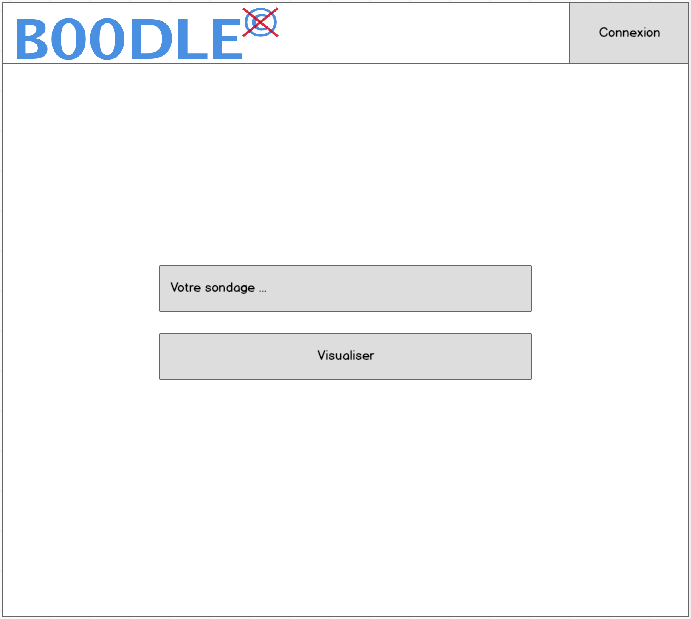
\includegraphics[scale=0.7]{figures/maquettes/accueil.png}
\end{figure}

\par Lorsque l'utilisateur accède à un sondage, il arrive sur la page principale (Dashboard) qui lui permet de consulter les caractéristiques et réponses actuelles du sondage. 
Ses propres réponses à ce sondage sont mises en évidence et il peut les éditer ou les supprimer. 
Il peut également ajouter une ou plusieurs réponses sur cette page (Figure \ref{maquette_dashboard}).
\par Cette page permet aussi à l'utilisateur de chatter avec les autres utilisateurs ayant accès à ce sondage.

\begin{figure}[h]
	\caption{Maquette - Dashboard}
	\label{maquette_dashboard}
	\centering
	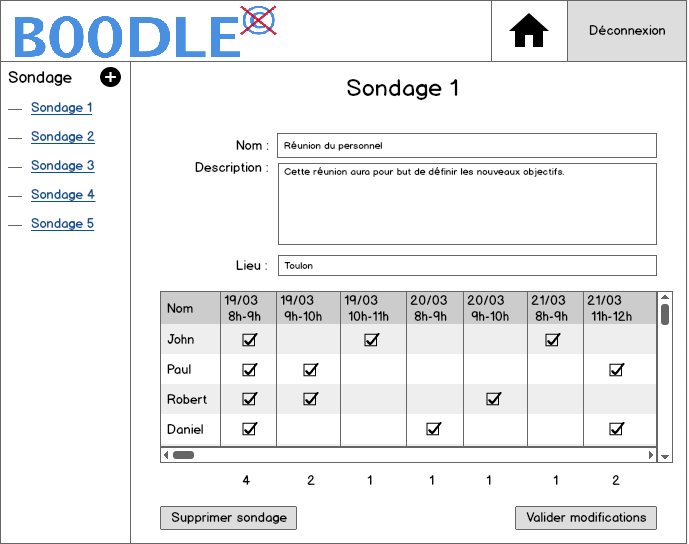
\includegraphics[scale=0.7]{figures/maquettes/dashboard.png}
\end{figure}

\paragraph{} Si l'utilisateur souhaite se connecter, il accède à une fenêtre l'invitant à rentrer ses identifiants (Figure \ref{maquette_connexion}). 
S'il ne possède pas de compte, il peut en créer en suivant le lien Créer un compte (Figure \ref{maquette_creationCompte}).

\begin{figure}[h]
	\caption{Maquette - Connexion}
	\label{maquette_connexion}
	\centering
	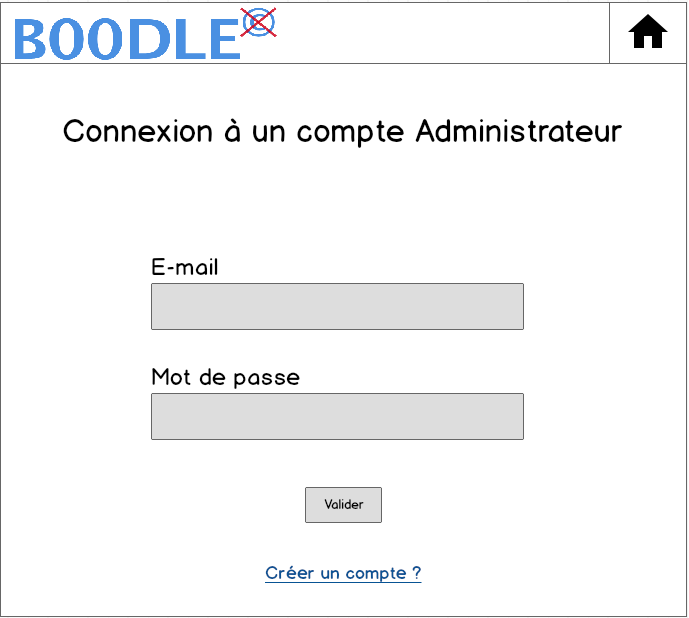
\includegraphics[scale=0.7]{figures/maquettes/connexion.png}
\end{figure}

\begin{figure}[h]
	\caption{Maquette - Créer un compte}
	\label{maquette_creationCompte}
	\centering
	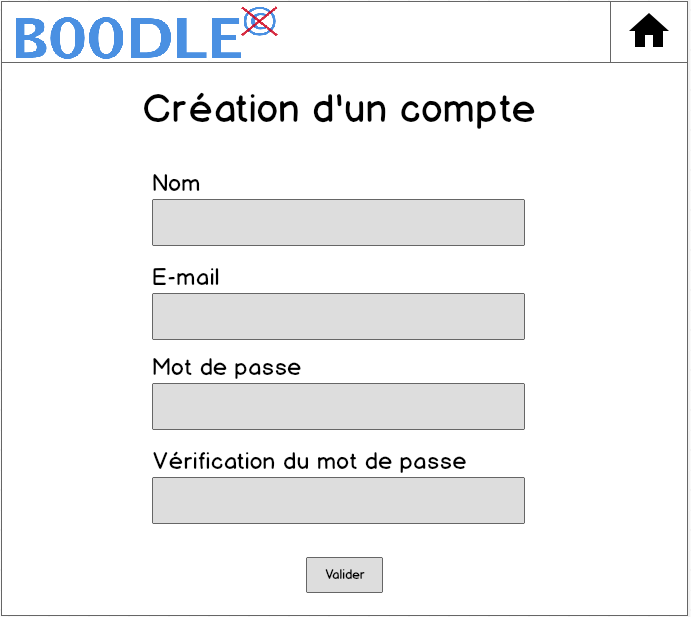
\includegraphics[scale=0.7]{figures/maquettes/creationCompte.png}
\end{figure}

\paragraph{} Une fois connecté, l'utilisateur peut accéder à la page de création de sondage (Figure \ref{maquette_creationEvenement}) afin d'entrer toutes les informations nécessaires à la création d'un nouveau sondage. 
Le bouton + à gauche permet d'accéder à la création de sondage depuis n'importe quelle page administrateur. 
Le bouton + en bas permet de valider le champ de texte de jour et d'ajouter une nouvelle date au sondage.

\begin{figure}[h]
	\caption{Maquette - Créer un sondage}
	\label{maquette_creationEvenement}
	\centering
	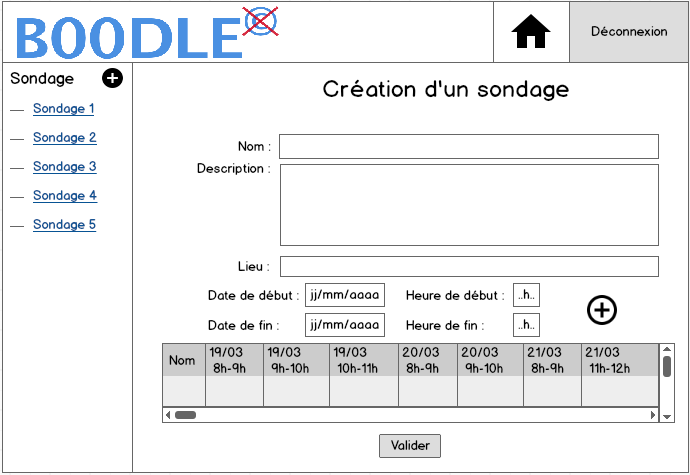
\includegraphics[scale=0.7]{figures/maquettes/creationEvenement.png}
\end{figure}

\paragraph{}Une fois la création validée, un popup permet de choisir les personnes à qui le logiciel va envoyer un mail les invitant à répondre au sondage (Figure \ref{maquette_popupAddParticipants}). 
Le bouton + permet de valider le champ de texte de l'adresse mail et d'envoyer un mail contenant le lien du sondage si l'adresse indiquée est valide.

\begin{figure}[h]
	\caption{Maquette - Ajouter des collaborateurs}
	\label{maquette_popupAddParticipants}
	\centering
	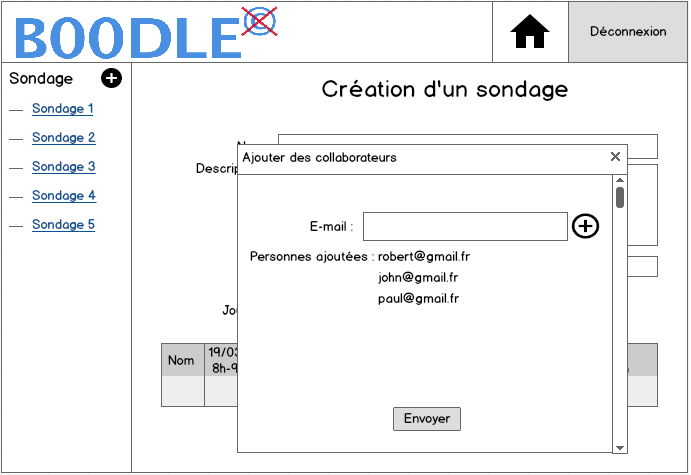
\includegraphics[scale=0.7]{figures/maquettes/popupAddParticipants.png}
\end{figure}

\paragraph{}En cliquant sur un sondage existant depuis l'interface administrateur, il est possible d'éditer certaines informations si l'administrateur est le créateur du sondage (Figure \ref{maquette_modifierEvenement}).

\begin{figure}[h]
	\caption{Maquette - Modifier un sondage}
	\label{maquette_modifierEvenement}
	\centering
	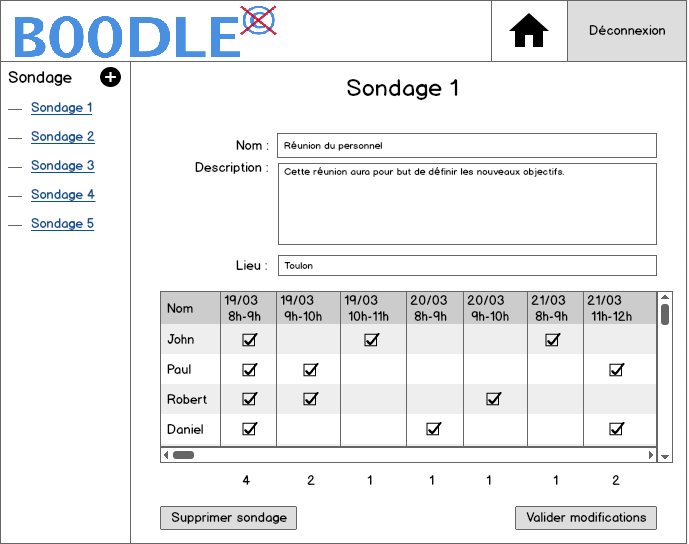
\includegraphics[scale=0.7]{figures/maquettes/modifierEvenement.png}
\end{figure}

\paragraph{}Depuis toutes les pages du logiciel, l'administrateur peut se déconnecter pour accéder à la page d'accueil.
\par Les cas nominaux d'utilisation utiliseront la navigation présentés dans le diagramme de navigabilité présenté en figure \ref{diagramme_navigabilite}. L'interface permettra également une navigation aisée entre les principales vues du logiciel. 
Par exemple, il sera possible d'accéder à l'accueil ou de se connecter/déconnecter depuis n'importe quelle vue du logiciel.

\begin{figure}[h]
	\caption{Diagramme de navigabilité}
	\label{diagramme_navigabilite}
	\centering
	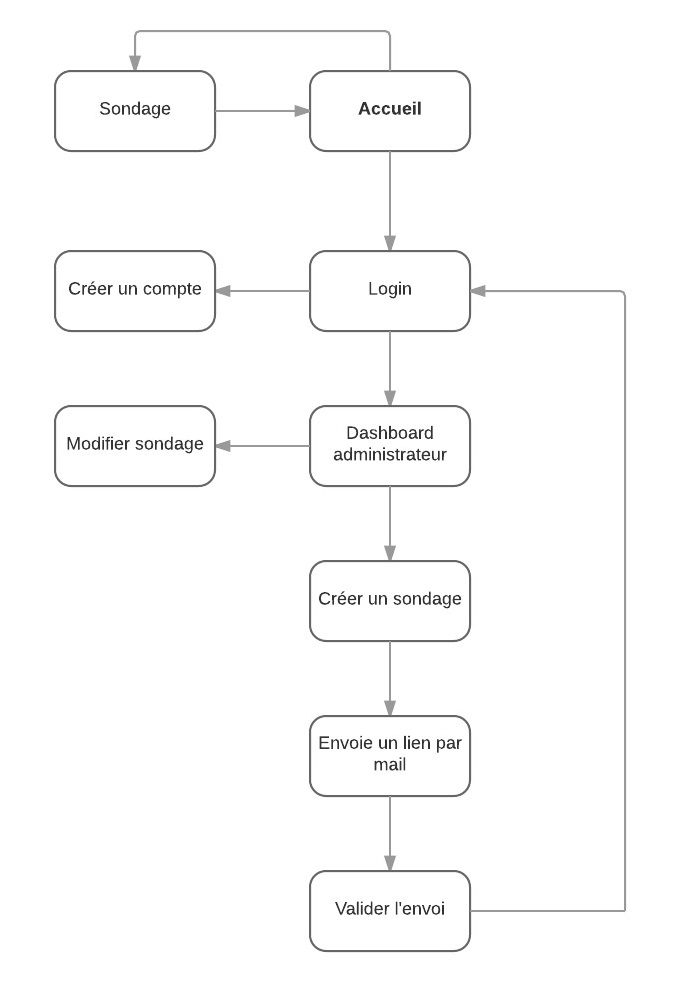
\includegraphics[scale=1]{figures/diagrammes/navigabilite.png}
\end{figure}

\clearpage

\chapter{Conception UML}

La modélisation UML présentée ici se concentrera principalement sur le fonctionnement du client. 
L'architecture du serveur sera détaillée dans la partie \ref{part_modelServer} (page \pageref{part_modelServer}). 
\par Dans cette partie, nous avons choisit de ne faire apparaître qu'une partie des diagrammes afin d'appuyer notre propos. 
La totalité des diagrammes UML utilisés lors de la conception de B00DLE sont présentés en partie \ref{part_allUML} (page \pageref{part_allUML}).

\section{Modélisation de l'axe statique}

\subsection{Diagramme de contexte statique}

Nous distinguons deux types d'acteurs, un utilisateur et un administrateur qui auront des utilisations du logiciel complètement distincts. 
Cette séparation nous permet d'autoriser une utilisation de l'application sans authentification pour l'utilisateur (\ref{diagramme_contexteStatique}). 

\begin{figure}[h]
	\caption{Diagramme de contexte statique}
	\label{diagramme_contexteStatique}
	\centering
	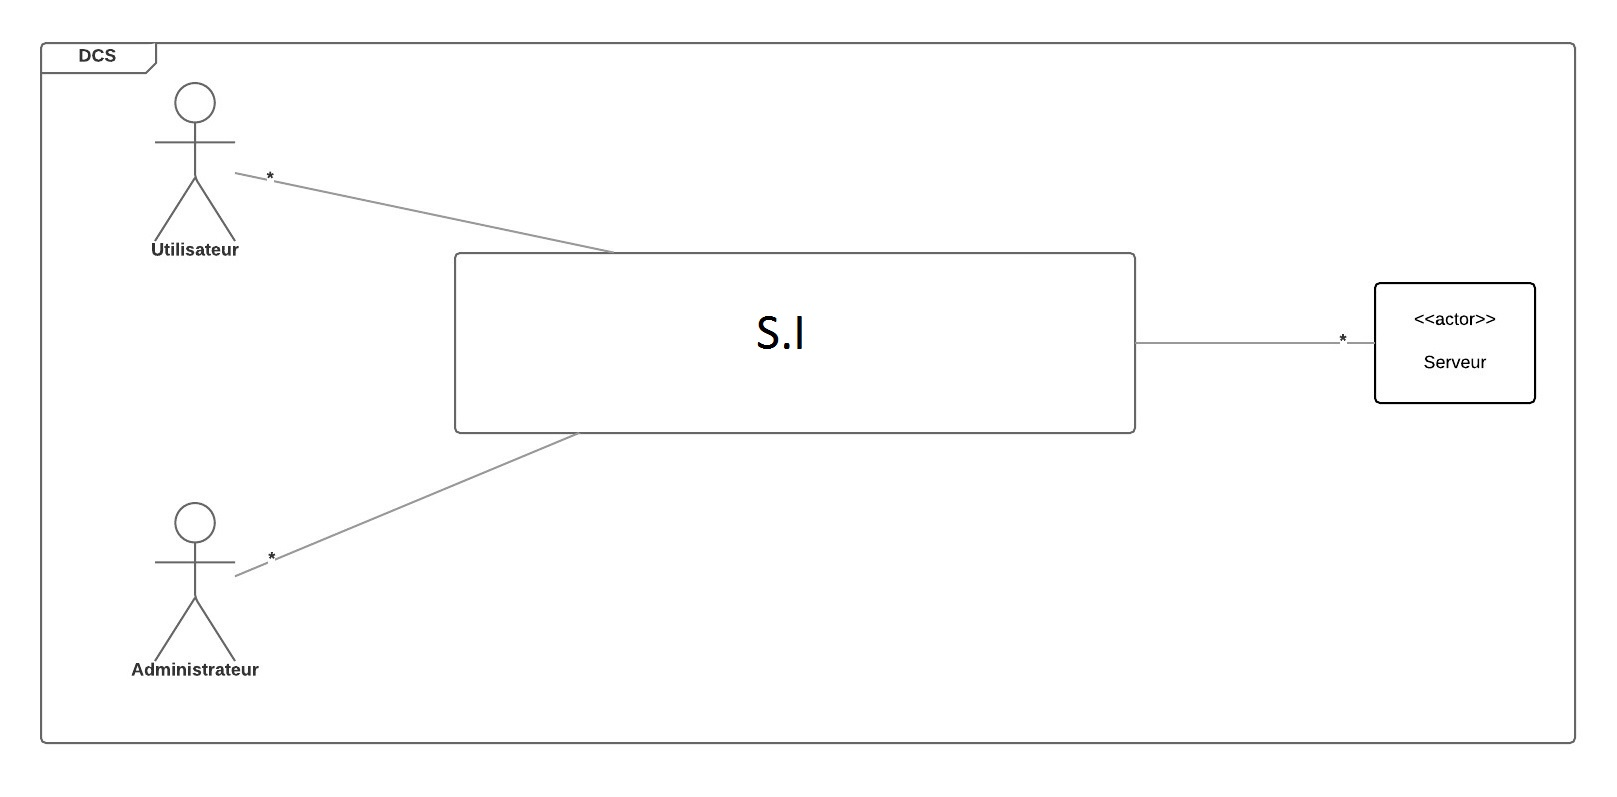
\includegraphics[scale=0.7]{figures/diagrammes/contexteStatique.png}
\end{figure}

L'accès aux données nécessaires au fonctionnement de B00DLE se fera par le biais d'un serveur codé en Ruby dont le fonctionnement est détaillé en annexe. C'est ce serveur qui communiquera avec la base de données.

\subsection{Diagramme des cas d'utilisation}

\par Les cas d'usage de l'administrateur requièrent tous une authentification. N'importe quel utilisateur peut créer un compte afin d'accéder au rôle d'administrateur après authentification (\ref{diagramme_casDUtilisation}).

\begin{figure}[h]
	\caption{Diagramme des cas d'utilisation}
	\label{diagramme_casDUtilisation}
	\centering
	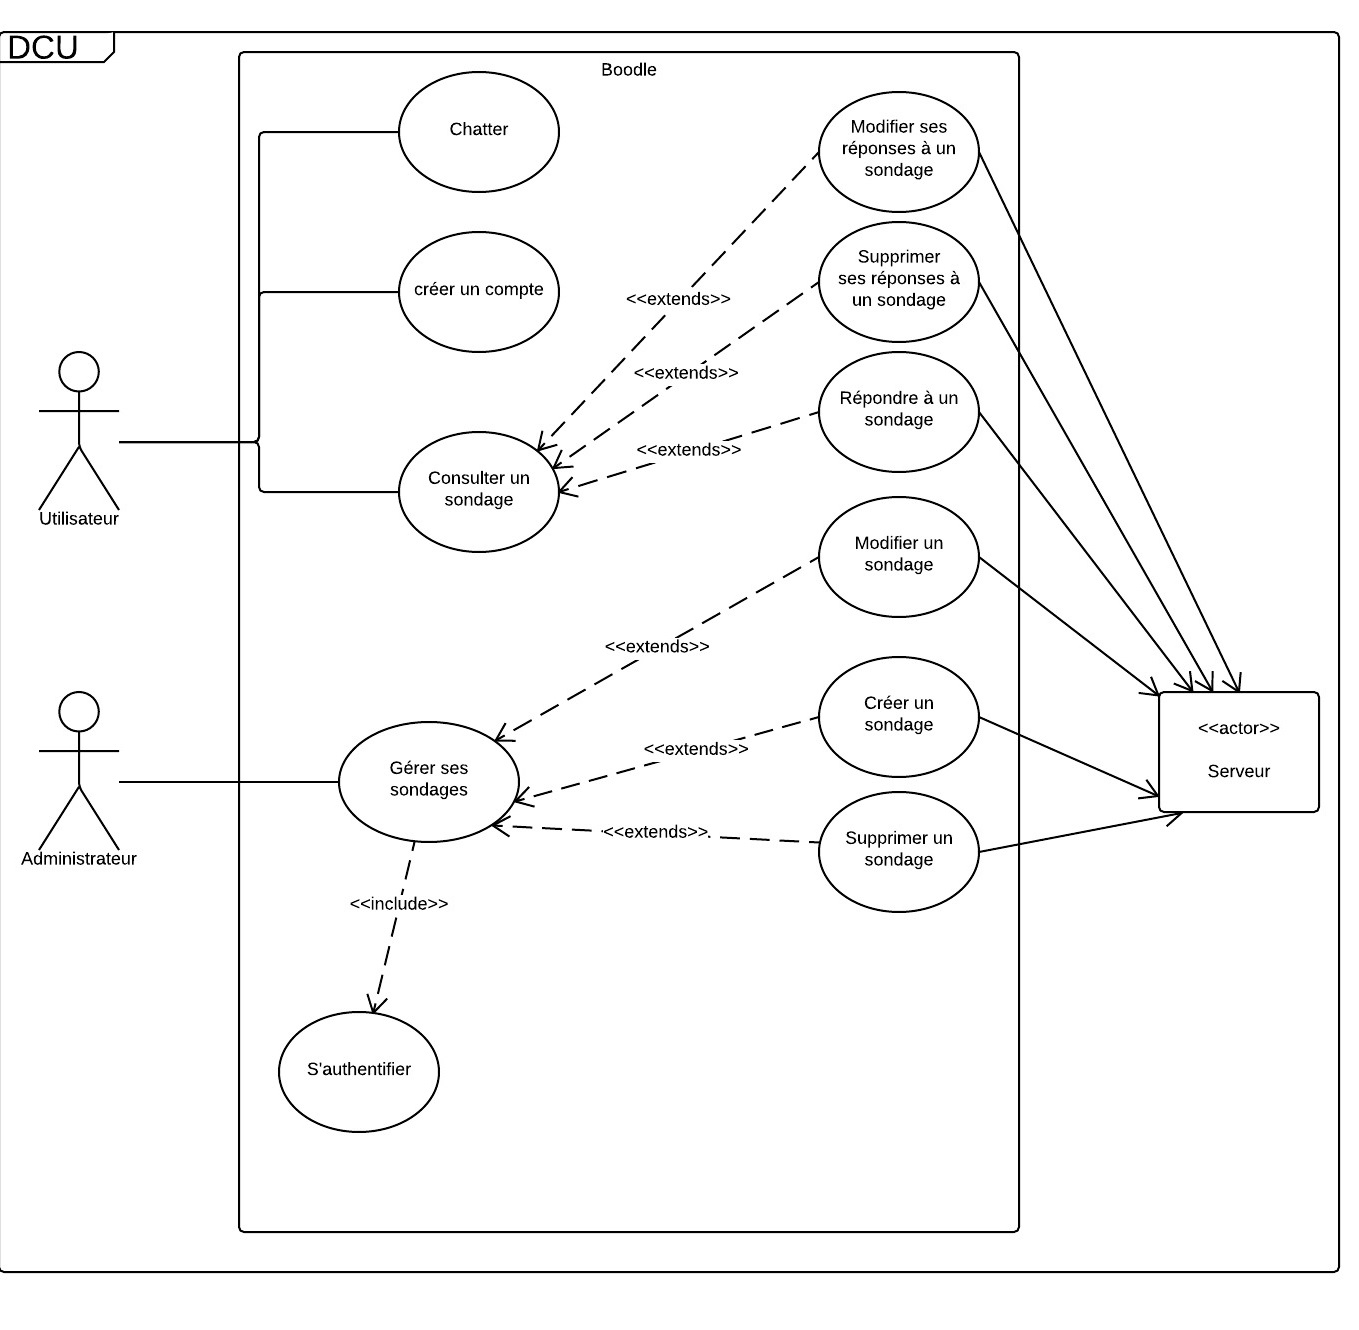
\includegraphics[scale=0.8]{figures/diagrammes/casDUtilisation.png}
\end{figure}

\par La priorité des cas d'utilisation est détaillée dans la figure \ref{tableau_casDUtilisation}. La principale fonctionnalité du logiciel est d'assurer la possibilité de créer un sondage et d'y ajouter des réponses.

	\begin{figure}[h]
	\caption{Priorité des cas d'utilisation}
	\label{tableau_casDUtilisation}
	\centering
\begin{tabular}{|c|c|c|c|}
	\hline
	Nom & Priorité & Risque & Classement \\
	\hline
	Créer un sondage & Haut & Moyen & 1 \\
	Répondre à un sondage & Haut & Moyen & 2 \\
	Supprimer ses réponses à un sondage & Moyen & Haut & 3 \\
	Consulter un sondage & Haut & Bas & 4 \\
	Supprimer un sondage & Bas & Haut & 5 \\
	Modifier un sondage & Moyen & Moyen & 6 \\
	Modifier ses réponses à un sondage & Moyen & Moyen & 7 \\
	Créer un compte & Haut & Bas & 8 \\
	Clôturer un sondage & Bas & Bas & 9 \\
	Chatter & Bas & Bas & 10 \\
	\hline
\end{tabular}
\end{figure}

\subsection{Diagramme de classe}

\par Le rôle d'administrateur est limité à la gestion de sondage, c'est pourquoi il ne partage rien avec le rôle d'utilisateur. 
\par Chaque utilisateur sera identifié par l'adresse MAC de son ordinateur afin qu'il puisse modifier ou supprimer ses propres réponses même en ayant fermé le logiciel auparavant. 
Cependant, s'il accède à un sondage depuis un autre ordinateur, B00DLE le considérera comme un nouvel utilisateur. Nous avons ce choix car nous devions permettre une utilisation du logiciel sans authentification.

\begin{figure}[h]
	\caption{Diagramme de classe}
	\label{diagramme_classes}
	\centering
	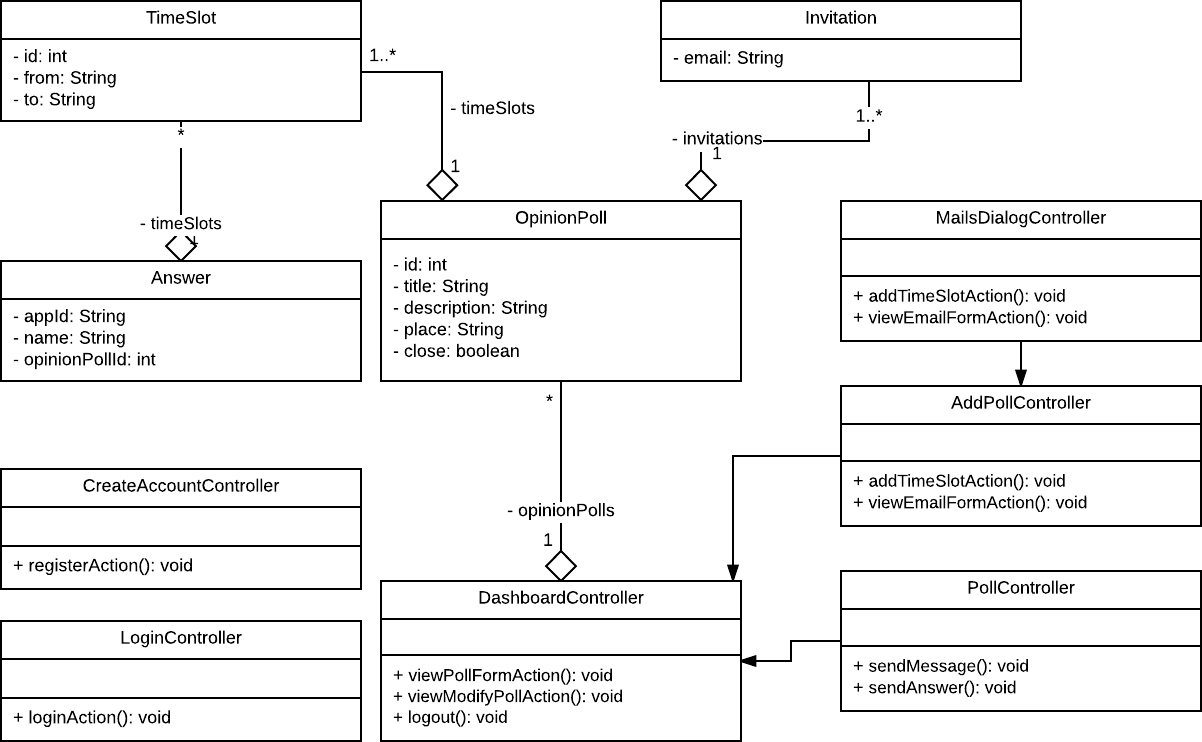
\includegraphics[width=\textwidth]{figures/diagrammes/classes.png}
\end{figure}

\par Notre application s'articule autour de la classe Sondage qui contient les informations liées au sondage. 
La base de données sur laquelle reposera notre application sera structurée selon le modèle fourni par ce diagramme de classe. 
Le diagramme entité association détaillé de cette base de données est présenté sur la figure \ref{diagramme_entiteAssociation}.

\begin{figure}[h]
	\caption{Diagramme entité-association}
	\label{diagramme_entiteAssociation}
	\centering
	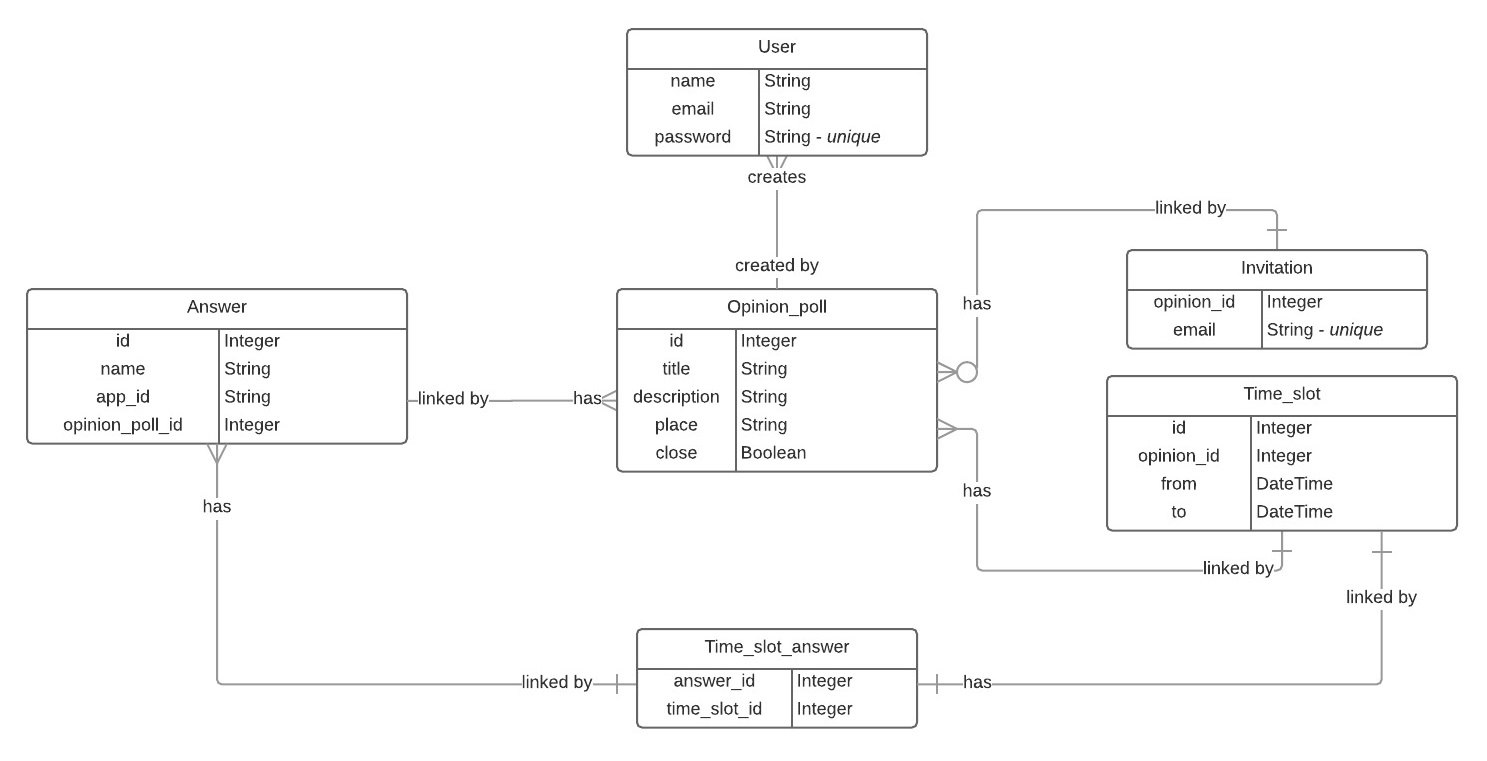
\includegraphics[width=\textwidth]{figures/diagrammes/entiteAssociation.png}
\end{figure}

\par Le serveur assurera la communication entre cette base de données et le client B00DLE.

\clearpage

\section{Modélisation des axes fonctionnel et dynamique}

\subsection{Généralités}

\par Tous les diagrammes de séquence et d'activité présentés ci-dessous seront depuis le point de vue du client.
\par Une rapide modélisation du serveur sera présentée dans la partie \ref{part_shortModelServer} (page \pageref{shortModelServer}). Les diagrammes de séquence client font pour la plupart référence au diagramme de séquence présenté figure \ref{diagramme_sequence_serveur} page \pageref{diagramme_sequence_serveur}.

\paragraph{} Tous les cas d'utilisation d'administration débutent par une connexion de l'utilisateur, décrite dans le diagramme de séquence en figure \ref{diagramme_sequence_connexion}. Ce diagramme illustre notre choix de déléguer tout le traitement et toute la vérification des données à notre serveur.

\begin{figure}[h]
	\caption{Diagramme de séquence - Connexion}
	\label{diagramme_sequence_connexion}
	\centering
	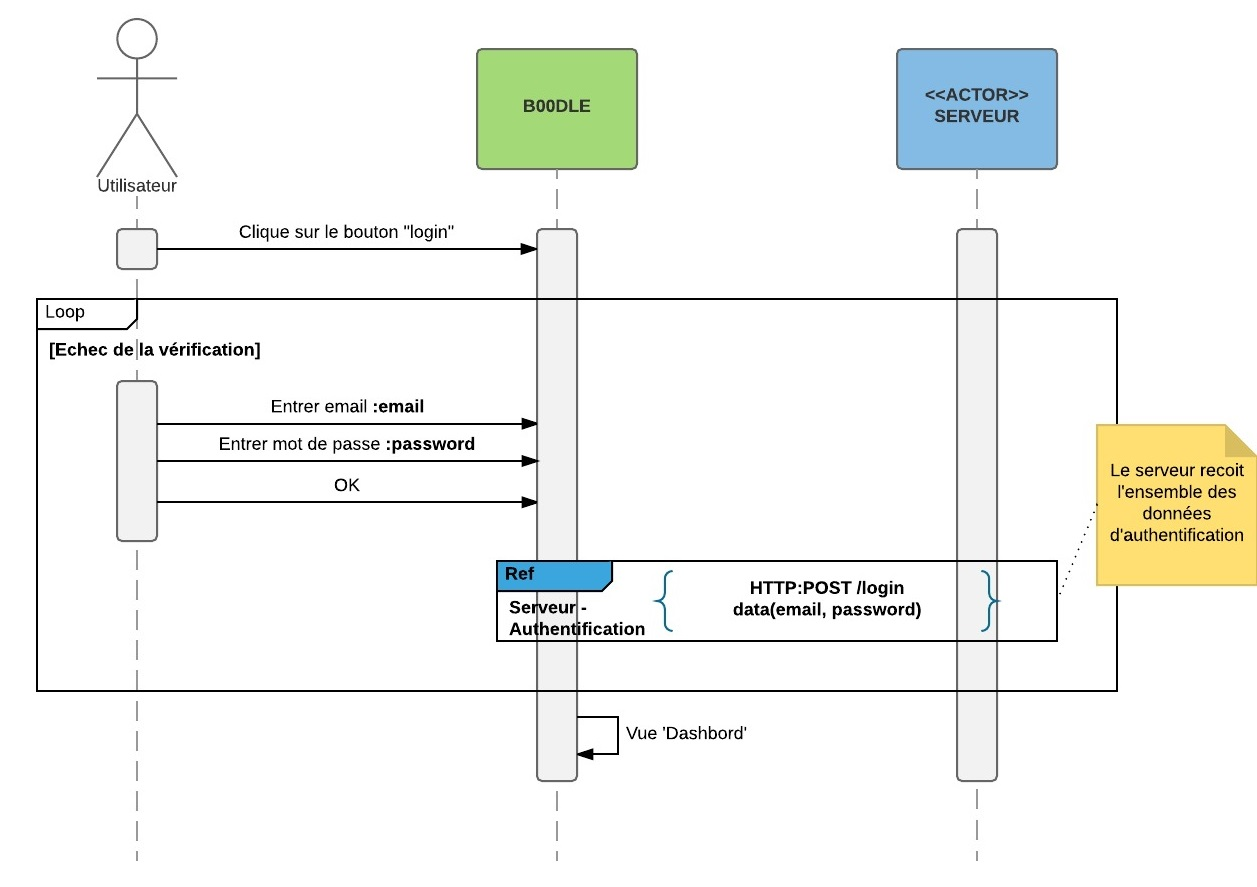
\includegraphics[width=\textwidth]{figures/diagrammes/sequence_connexion.png}
\end{figure}

\par Avant sa première connexion, l'utilisateur devra créer un compte pour obtenir ses informations de connexion (diagramme de séquence figure \ref{diagramme_sequence_inscription}). Là encore, on peut remarquer que le client n'effectue aucun traitement sur les données entrées par l'utilisateur.

\begin{figure}[h]
	\caption{Diagramme de séquence - Inscription}
	\label{diagramme_sequence_inscription}
	\centering
	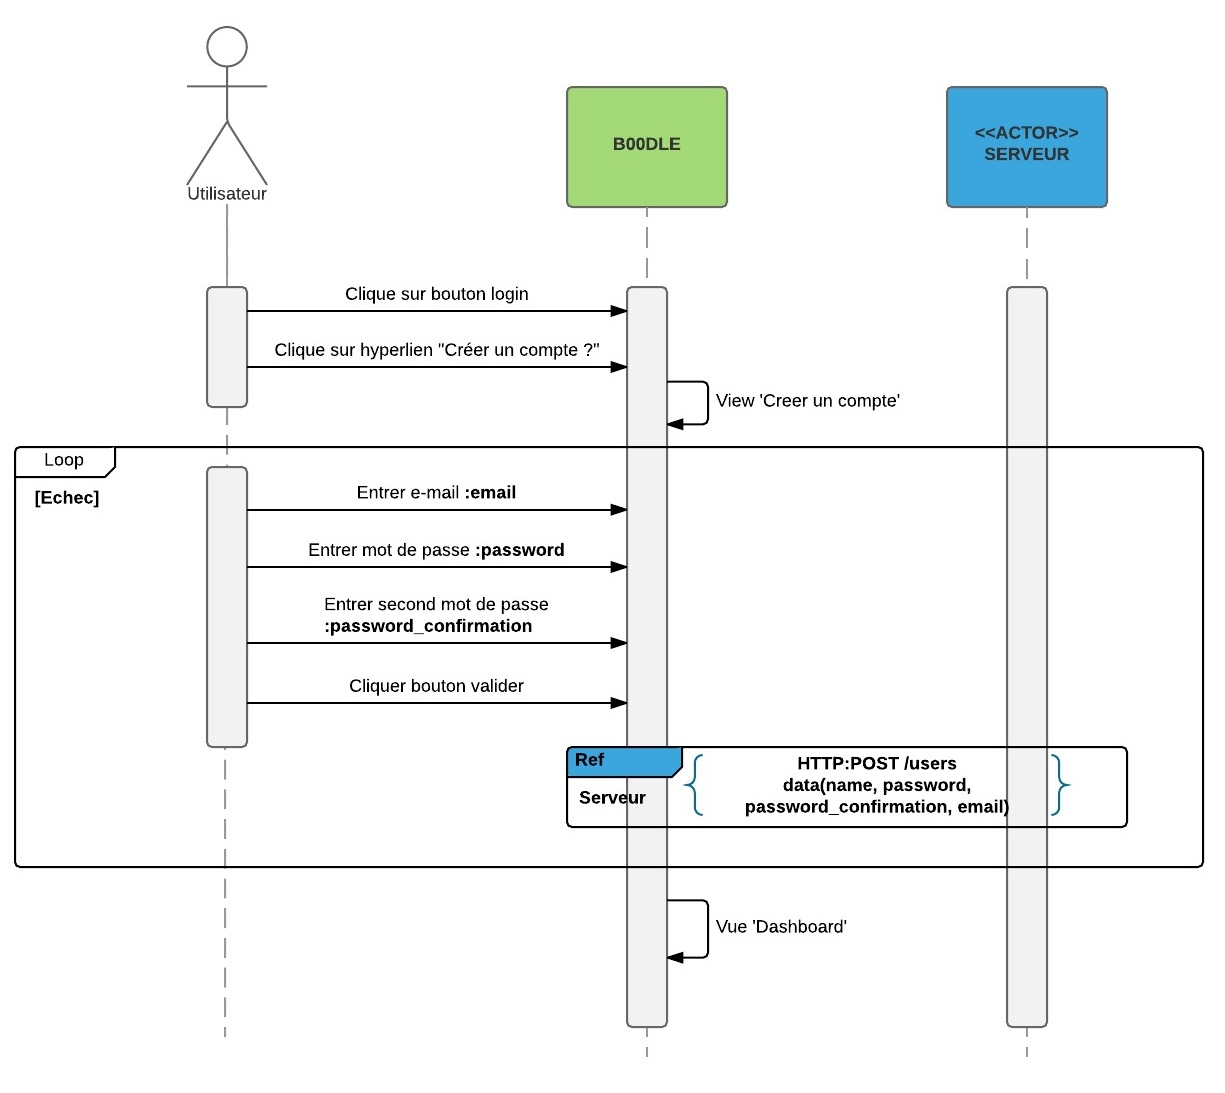
\includegraphics[width=\textwidth]{figures/diagrammes/sequence_inscription.png}
\end{figure}

\clearpage

\subsection{Traitement d'un cas d'utilisation - Créer un sondage}

\paragraph{} Le cas d'utilisation que nous avons choisi de détailler ici est la création d'un sondage. C'est un des cas d'utilisation essentiel au fonctionnement de notre application et son modèle de fonctionnement est proche de celui des autres cas d'utilisation faisant intervenir un sondage.

\paragraph{} Le diagramme de séquence (figure \ref{diagramme_sequence_creerSondage}) s'articule principalement autour de trois étapes : authentification, saisie des données du sondage puis envoi des données aux serveur.

\begin{figure}[h]
	\caption{Diagramme de séquence - Créer un sondage}
	\label{diagramme_sequence_creerSondage}
	\centering
	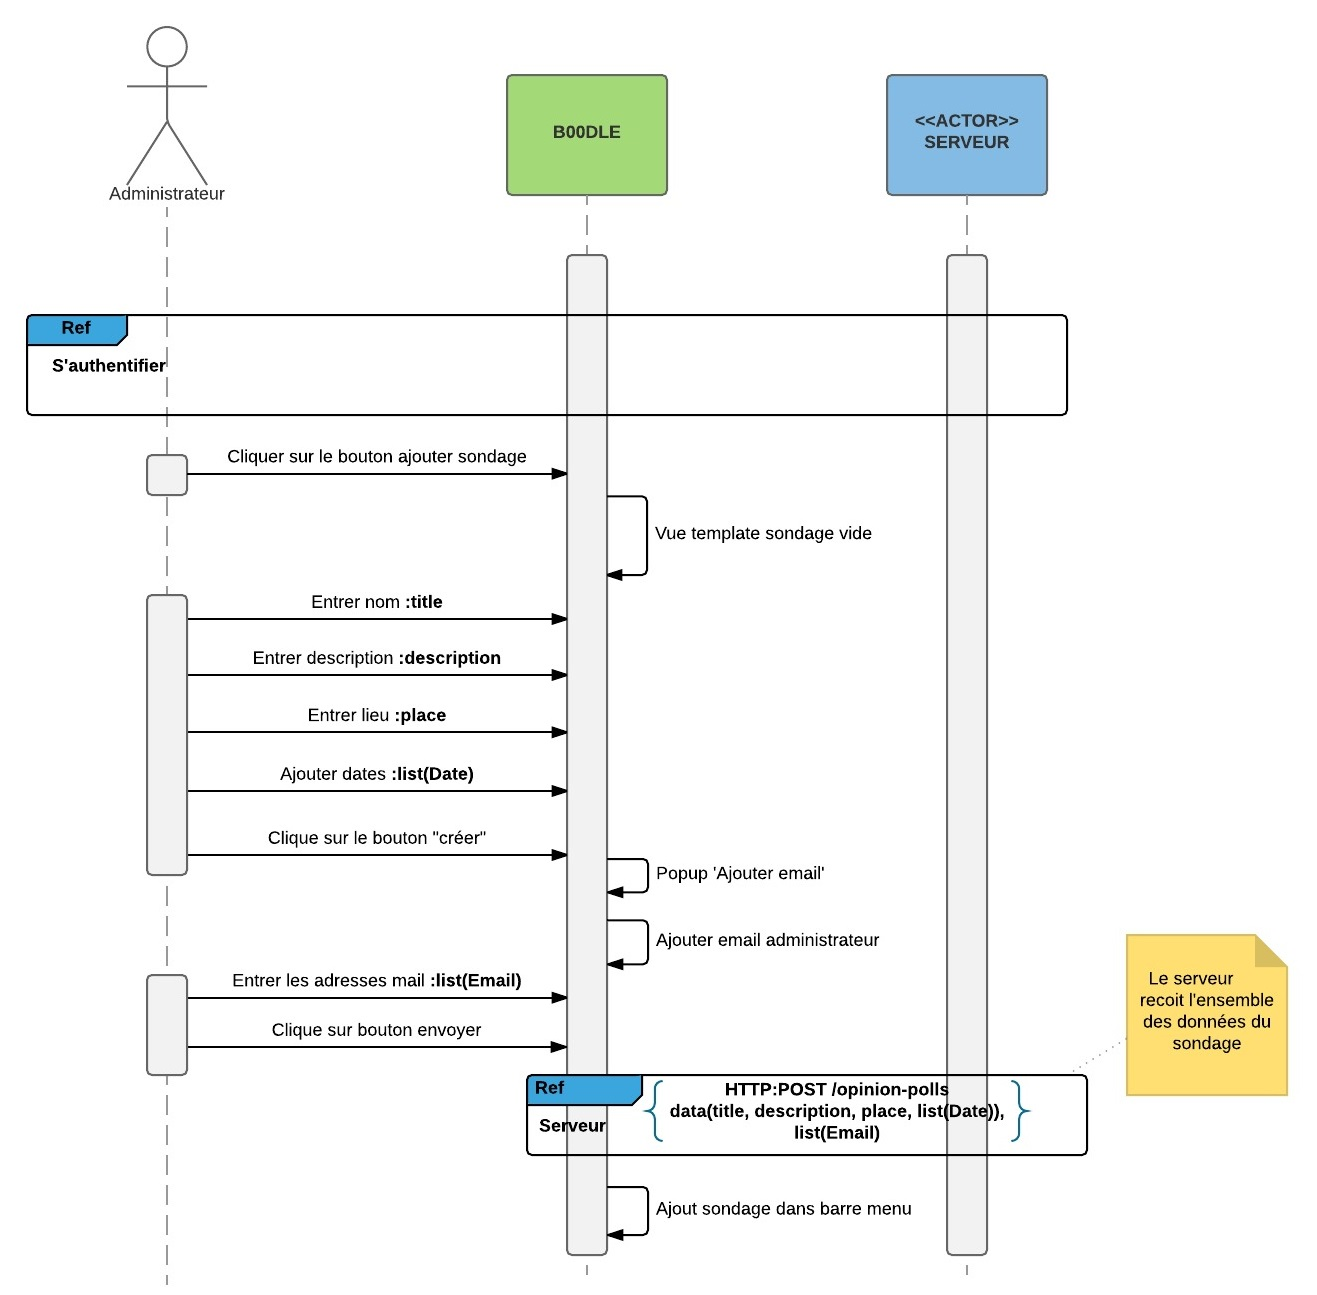
\includegraphics[width=\textwidth]{figures/diagrammes/sequence_creerSondage.png}
\end{figure}

\paragraph{} Comme on peut le voir sur le diagramme d'activité (figure \ref{diagramme_activite_creerSondage}), c'est le serveur qui se charge de remonter les erreurs sur le format des données ou sur la lecture/écriture en base de données. Le client ne fait qu'informer l'utilisateur sur l'échec de l'opération.

\begin{figure}[h]
	\caption{Diagramme d'activité - Créer un sondage}
	\label{diagramme_activite_creerSondage}
	\centering
	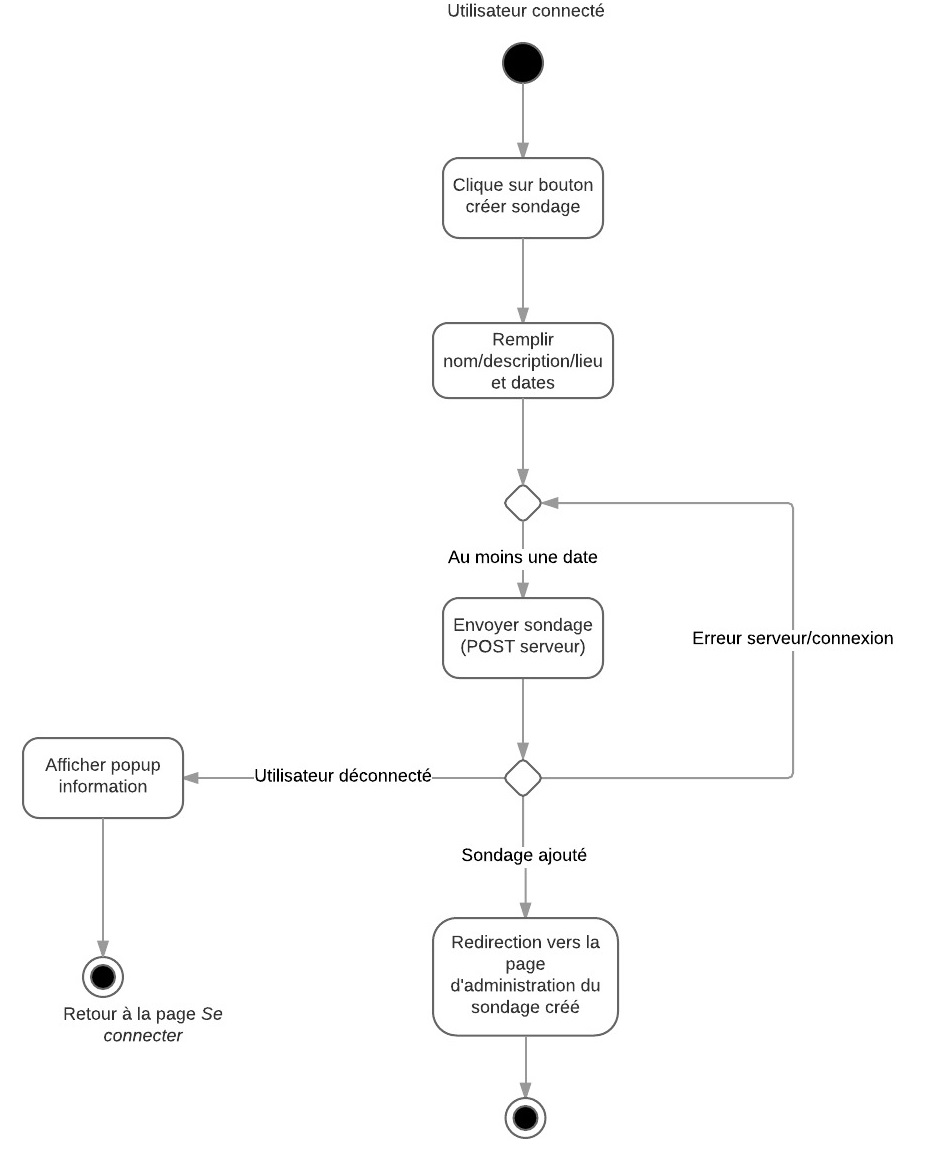
\includegraphics[scale=0.8]{figures/diagrammes/activite_creerSondage.png}
\end{figure}

\paragraph{} Les cas d'utilisation de suppression et modification de sondage sont très similaires (voir diagramme de séquence de modification de sondage figure \ref{diagramme_sequence_modifierSondage}).

\begin{figure}[h]
	\caption{Diagramme de séquence - Modifier un sondage}
	\label{diagramme_sequence_modifierSondage}
	\centering
	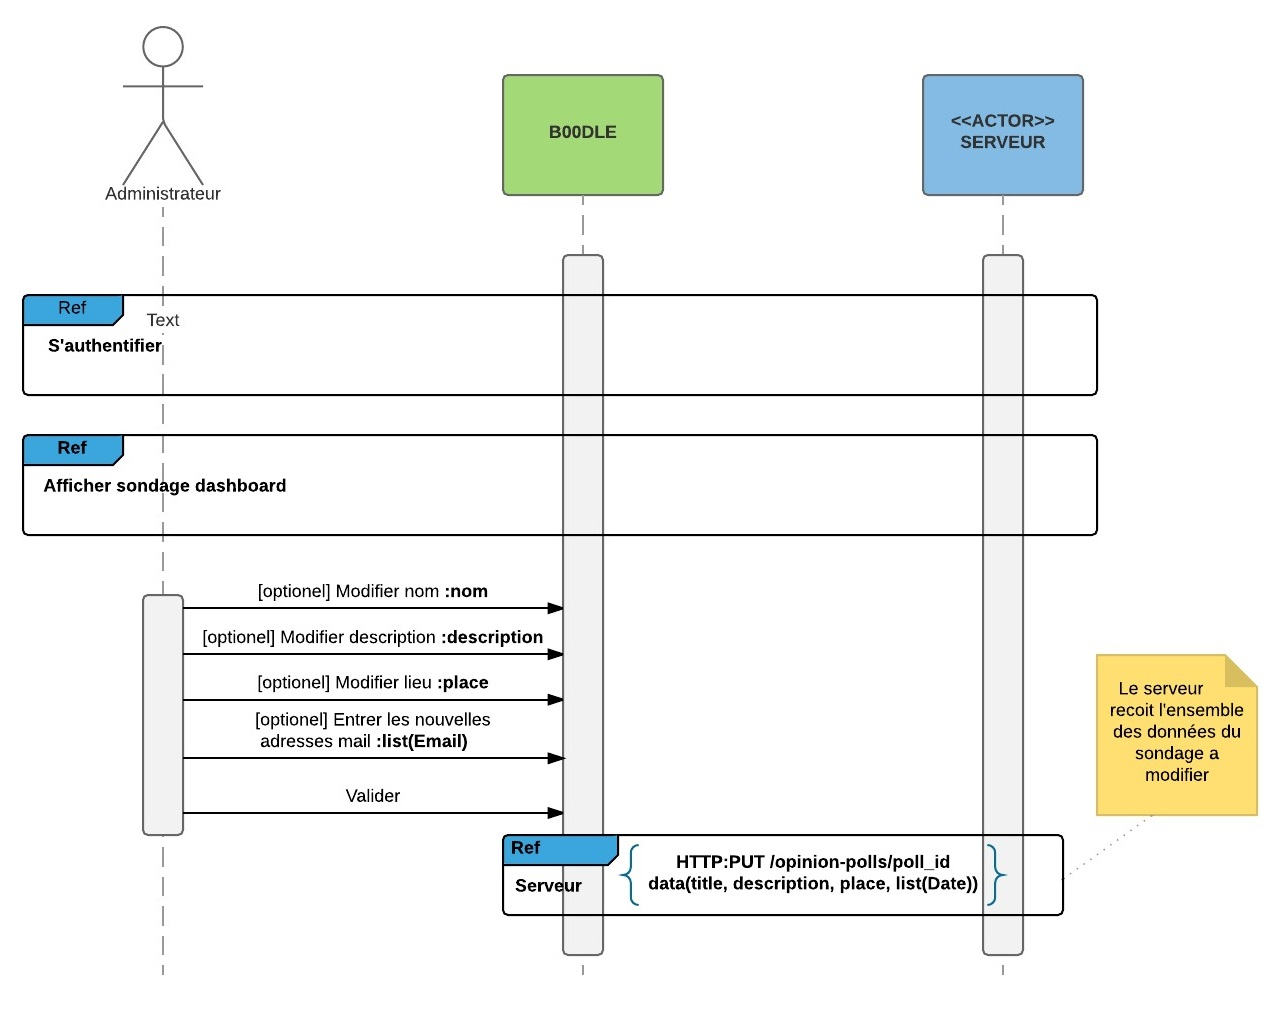
\includegraphics[width=\textwidth]{figures/diagrammes/sequence_modifierSondage.png}
\end{figure}

\clearpage

\subsection{Traitement d'un cas d'utilisation - Répondre à un sondage}


\begin{figure}[h]
	\caption{Diagramme de séquence - Répondre à un sondage}
	\label{diagramme_sequence_repondreSondage}
	\centering
	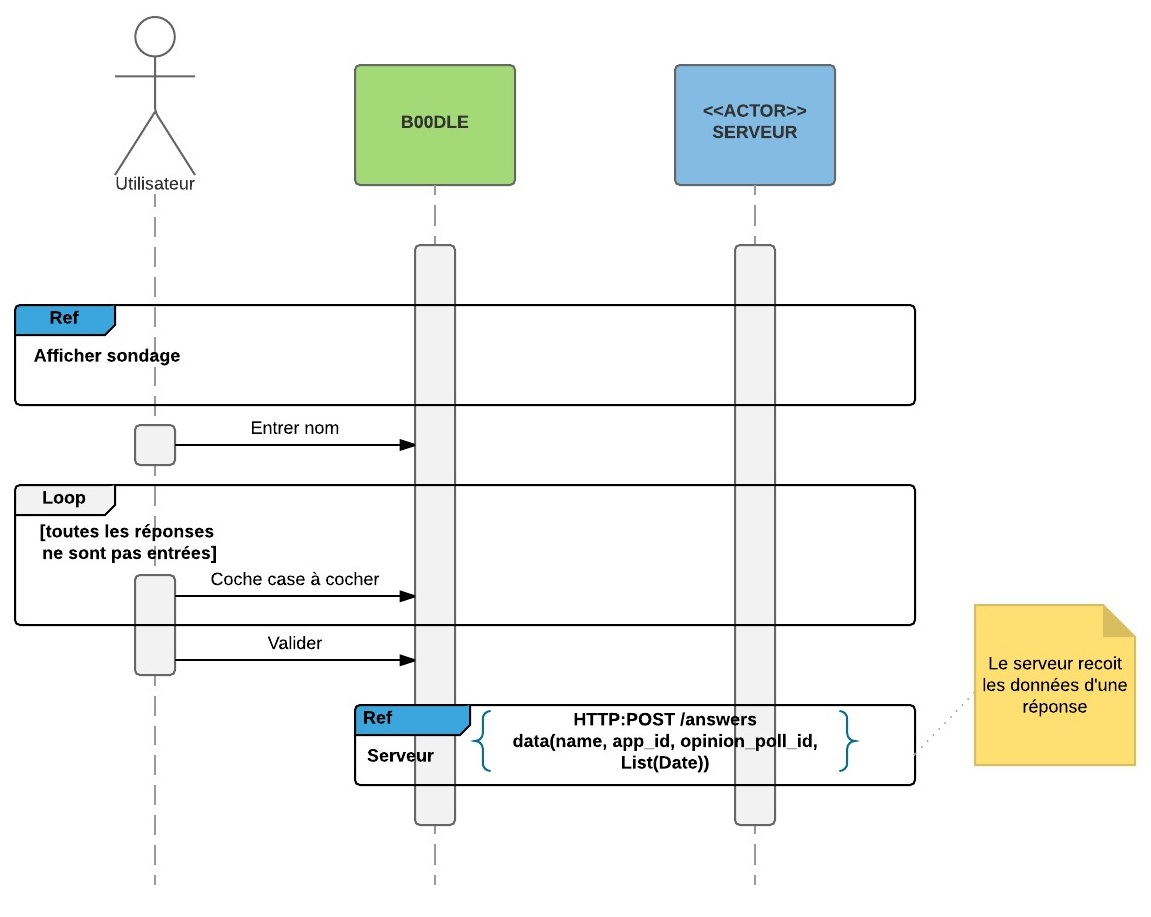
\includegraphics[width=\textwidth]{figures/diagrammes/sequence_repondreSondage.png}
\end{figure}

\begin{figure}[h]
	\caption{Diagramme d'activité - Répondre à un sondage}
	\label{diagramme_activite_répondreSondage}
	\centering
	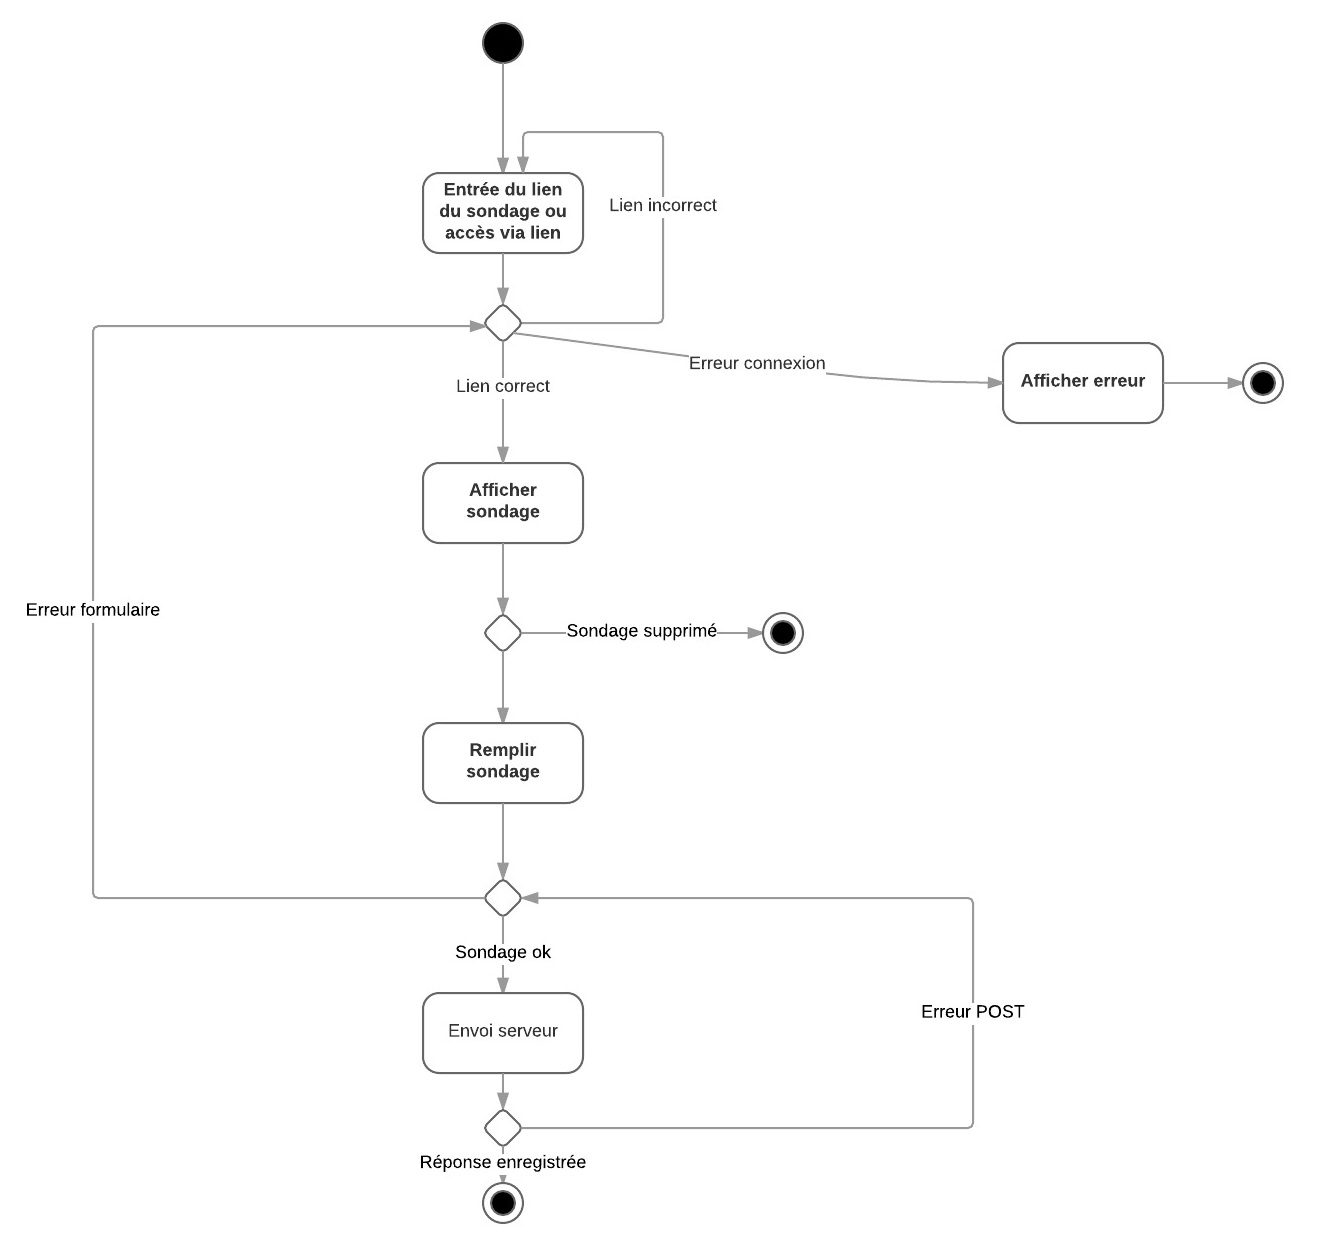
\includegraphics[scale=0.8]{figures/diagrammes/activite_repondreSondage.png}
\end{figure}


\clearpage

\section{Modélisation rapide du serveur} 
\label{part_shortModelServer}

\begin{figure}[h]
	\caption{Diagramme de séquence - Serveur}
	\label{diagramme_sequence_serveur}
	\centering
	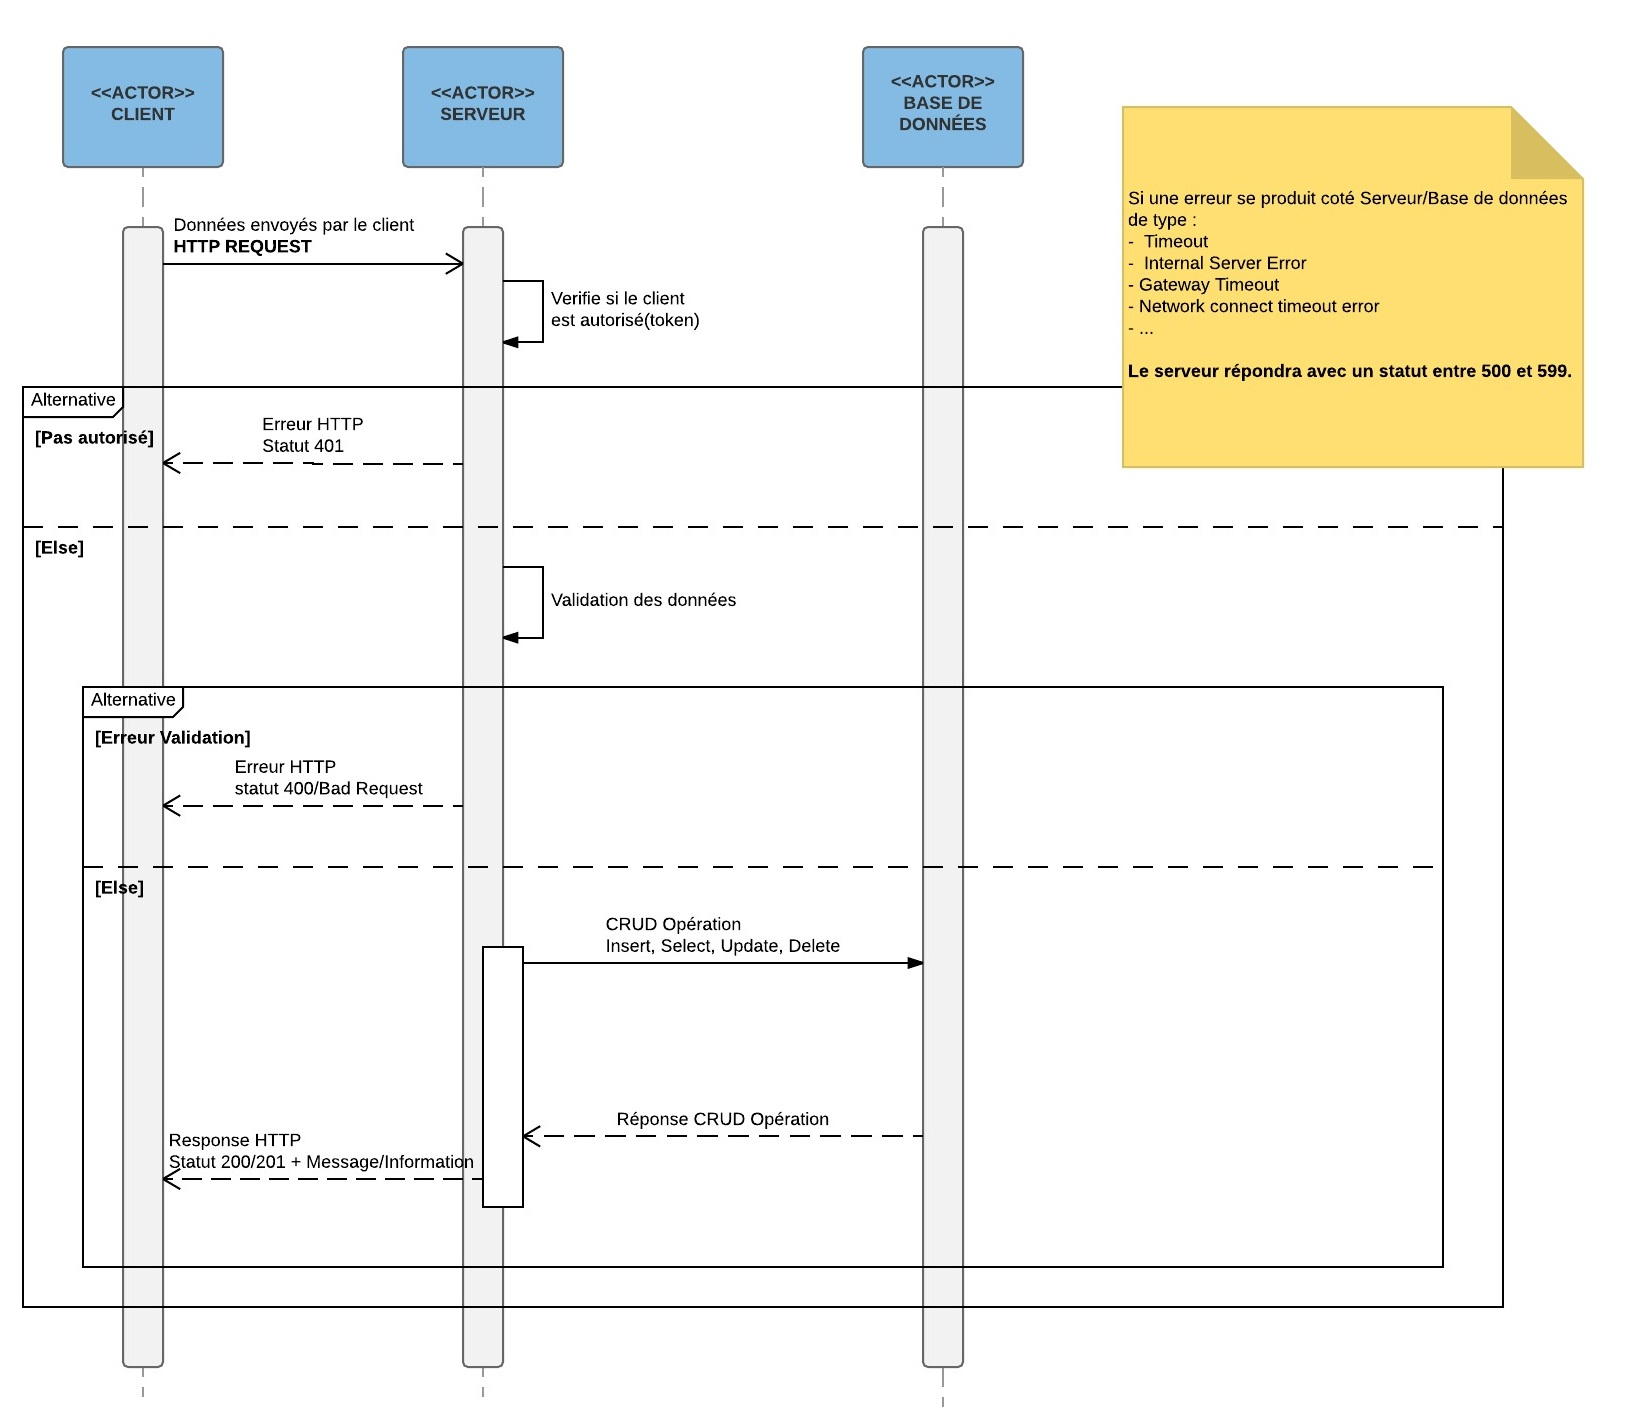
\includegraphics[width=\textwidth]{figures/diagrammes/sequence_serveur.png}
\end{figure}

\chapter{Implémentation}


\clearpage
\part{Modélisation serveur}
\label{part_modelServer}

\par TODO

\part{Diagrammes UML}
\label{part_allUML}

\par TODO

\end{document}          
